\documentclass{jcst}

% The IJCS template requires the following packages installed in your LaTeX2 distribution:
%etoolbox,microtype,lmodern,sectsty,graphicx,booktabs,geometry,amssymb,amsmath,amsthm,authblk

\title{Author's Guide for Preparing a Paper for the Journal of Computer Science \& Technology}

\author[1,2]{First Author}
\author[2]{Second Author}
\author[1]{Last Author}

% \authorcr produces a newline inside the \affil command
\affil[1]{University Department, University Name City, State ZIP/Zone, Country \authorcr
\{firstauthor, lastauthor\}@mail.dom }
\affil[2]{Another University Department, University Name City, State ZIP/Zone, Country \authorcr
\{secondauthor\}@mail.dom}

\begin{document}

\maketitle

\begin{abstract}
These instructions give you guidelines for preparing papers for the
Journal of Computer Science \& Technology. The abstract should summarize the
 content of the paper. Try to keep the abstract below 200 words. Do not make
  references nor display equations in the abstract. The journal will be printed
  by photo-offset from the same-sized copy prepared by you. Your manuscript
   should be printed on A4 paper (21.0 cm x 29.7 cm). It is imperative that the
 margins and style described below be adhered to carefully. This will enable
 us to keep uniformity in the final printed copies of the Journal. Please
 keep in mind that the manuscript you prepare will be photographed and
 printed as it is received. Readability of copy is of paramount importance.
\end{abstract}

\keywords{Enter key words or phrases in alphabetical order (5 maximum), separated by commas.}

\reception{Received 4 December 2014; Revised 7 May 2015; Accepted 17 June 2015}

\section{Important Information}

The submitted papers must be original. Do not submit a reworked version of a paper you
have submitted or published elsewhere. Do not publish preliminary data or results.
The submitting author is responsible for obtaining agreement of all coauthors and
any consent required from sponsors before submitting a paper. The authors must
 cite relevant prior work.
There is a limit of 7 pages for each paper in the Journal. Each submission should
be a .pdf file submitted through the JCS\&T management system.

\section{Preparations of manuscripts}

\subsection{General Appearance}

The text must be in English. The submitted typeset scripts of each contribution must be in their final form and of good appearance since they will be printed directly without any editing. It is essential that the \textit{camera-ready copies} be absolutely clean.
Your paper must be printed in two columns. Columns should be balanced in the last page. The document you are reading is printed in the format that should be used in your paper.

\subsection{Specification}

To ensure uniformity of appearance for the Journal, your paper should conform to
 the following specifications. If your paper deviates significantly from these
 specifications, the printer may not be able to include your paper in the Journal.

\begin{enumerate}
\item The top, bottom, left, and right margins should be 2.5 cm.
\item The distance between the two columns of text should be 1cm.
\end{enumerate}

\section{Font size}
The font size must be 10 points. This document is set in 10-point Times. Some technical
formatting programs print mathematical formulas in italic type, with subscripts
and superscripts in a slightly smaller or bigger font size. This is acceptable.
Major headings are to be column centered in a bold font without underline.
They must be numbered, and written all in caps. For example, the text
 \textbf{4. MAJOR HEADINGS} at the bottom of this paragraph is a major heading.

\section{Major headings}

\subsection{Subheadings}
Subheadings should be in a bold font lower case, with the first letter capitalized.
They should start at the left-hand margin on a separate line.

\subsection{Sub-subheadings}
Sub-subheadings are to be in a bold font. They are formatted as subheadings,
but they have no tag. The following is a sub-subsection.

 \subsubsection{A sample sub-subheading}
 This sub-subsection's heading has no tag.

\section{Illustrations}

The illustrations can be in color. However, because printed version will be in
 black and white, you must ensure a clear view in grayscale. All illustrations
 must have a DPI of 200 or more. The caption must be placed \textit{after} the
 graphic.

\begin{figure}
\label{sample}
\centering
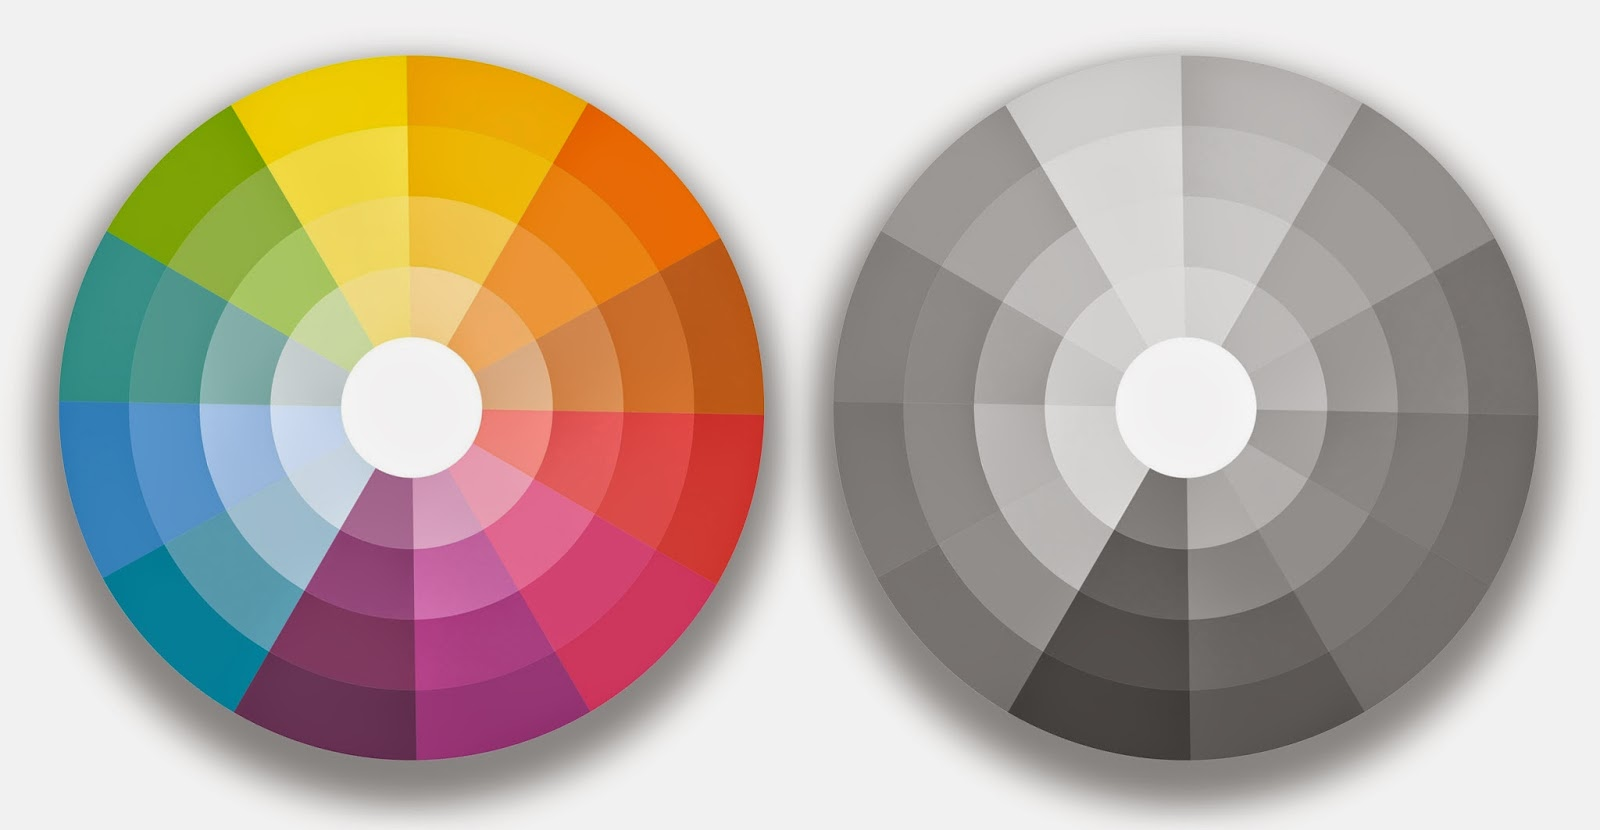
\includegraphics[width=0.4\textwidth]{colors}
\caption{Sample image}
\end{figure}

\section{Formulae}
All equations must be typed or written neatly in black. They should be numbered
consecutively throughout the text. Equation numbers should be enclosed in
parentheses and flushed right. Equations should be referred to as Eq \eqref{eq:sample}
in the text where $1$ in this case is the equation number.

 \begin{equation}
   \label{eq:sample}
   (1+x)^n=1+\frac{nx}{1!}+\frac{n (n-1) x^2}{2!}+\dots
 \end{equation}

 In multiple-line equations, the number should be given on the last line.

\begin{align}
\label{eq:aligned}
(1+x)^n&=1+\frac{nx}{1!}+\frac{n (n-1) x^2}{2!}+\dots \notag
      \\&=\sum_{i=0}^{n} {n\choose i} x^i
 \end{align}

 If you are using Word, use either the Microsoft Equation Editor or the MathType add-on
(http://www.mathtype.com) for equations in your paper. If you are using LaTeX, the
AMS mathematical packages are highly recommended for typesetting complex formulas.

\section{Tables}

Tables must be in black and white. The caption must be placed before the table,
and is obligatory. The table must not contain vertical lines or borders.

\begin{table}[tp]
\caption{Sample table}
\label{sampletable}
\centering
\begin{tabular}{clccc}
\toprule
$D$ &               & $P_u$      & $\sigma_N$    \\
(in)&               & (lbs)      & (psi)          \\ \otoprule
%
5    & test 1      & 285         & 38.00          \\
& test 2      & 287         & 38.27          \\
& test 3      & 230         & 30.67          \\ \midrule
10   & test 1      & 430         & 28.67          \\
& test 2      & 433         & 28.87          \\
& test 3      & 431         & 28.73          \\ \bottomrule
\end{tabular}
\end{table}

\section{Page numbering}
Please do NOT number your pages.

\section{Foot notes}
Should be typed in singled-line spacing at the bottom of the page and column where it is cited. Footnotes should be rare.

\section{Conclusions}
The better you look, the better we all look. Thanks for your cooperation and contribution

\section{References}
List and number all bibliographical references at the end of your paper.
When referenced in the text, enclose the citation  number in square brackets,
for example \cite{article} or \cite{phdthesis},\cite{unpublished},\cite{book},\cite{proceedings},\cite{mastersthesis}. The preferred citing package in LaTeX is bibtex.

\acknowledgements{
This paragraph is meant for acknowledgements and support information.
}

\bibliography{references}

\end{document}
